\documentclass[final,t]{beamer}
\mode<presentation>
{
	\usetheme{boxes}
}

\usepackage[orientation=portrait,size=a1,scale=1,debug]{beamerposter}
\usepackage{graphicx}
\usepackage{setspace}
\usepackage{tabularx}
\usepackage{tikzsymbols}
\usepackage{tikz}
\usepackage{spot}
\usepackage{tabularx}
%\usepackage[table]{xcolor}
\usepackage[absolute,overlay]{textpos}
\usepackage{booktabs}
\usepackage{subcaption}
\usepackage{lipsum} % for dummy text
\usepackage{color, colortbl} %righe colorate

\setbeamerfont{subtitle}{size=\large, series=\bfseries}
\definecolor{template}{RGB}{181, 18, 27}
\setbeamercolor{frametitle}{fg=template, bg=white}
\setbeamercolor{section in head/foot}{bg=template}
\setbeamercolor{subsection in head/foot}{bg=template!20, fg=template}
\setbeamercolor{author in head/foot}{bg=template}
\setbeamercolor{date in head/foot}{fg=template}
\setbeamercolor{title in head/foot}{fg=template}
\setbeamercolor{title}{fg=template}
\setbeamercolor*{item}{fg=template}
\setbeamercolor{block title}{bg=white, fg=template}
\setbeamertemplate{frametitle}[default][center]
\setbeamertemplate{caption}[numbered]

\definecolor{back}{RGB}{247, 251, 255}
\definecolor{map}{RGB}{111, 172, 232}
\definecolor{childmap}{RGB}{161, 200, 240}
\definecolor{nodemap}{RGB}{141, 170, 199}
\definecolor{rasch}{rgb}{0.0, 0.33, 0.71}
\definecolor{log}{rgb}{0.0, 0.65, 0.58}
\definecolor{diff}{RGB}{33, 113, 181}
\definecolor{single}{RGB}{106, 81, 163}
\definecolor{comp}{RGB}{35, 99, 70}
\definecolor{inc}{RGB}{191, 13, 43}
\definecolor{highlight}{rgb}{0.45, 0.31, 0.59}
\definecolor{section}{RGB}{51,51,179}
\definecolor{typical}{RGB}{8, 69, 148}
\definecolor{model}{RGB}{74, 20, 134}
\definecolor{orangered2}{RGB}{238,64,0}
\definecolor{royalblue3}{RGB}{58,95,205}
\definecolor{springgreen}{RGB}{0,205,102}
\definecolor{magenta}{RGB}{255,0,255}
\definecolor{seagreen}{RGB}{75, 155, 110}

\setbeamercolor{frametitle}{fg=template, bg=white}
\setbeamercolor{section in head/foot}{bg=template}
\setbeamercolor{subsection in head/foot}{bg=template!20, fg=template}
\setbeamercolor{author in head/foot}{bg=template}
\setbeamercolor{date in head/foot}{fg=template}
\setbeamercolor{title in head/foot}{fg=template}
\setbeamercolor{title}{fg=template}
\setbeamercolor*{item}{fg=template}
\setbeamertemplate{frametitle}[default][center]

\title[Pauci sed moni]{\huge Pauci sed moni: \\ An item response theory approach for shortening tests}
\author[]{\large \textbf{Ottavia M. Epifania}\textsuperscript{1,2} \and Pasquale Anselmi\textsuperscript{1} \and Egidio Robusto \textsuperscript{1}}
\institute[]{\large \textsuperscript{1} University of Padua \\ \textsuperscript{2}Catholic University of the Sacred Heart }
\date{ottavia.epifania@unipd.it}


\begin{document}
		\vspace{5mm}
	
	
	\begin{frame}
\begin{textblock*}{5cm}(2cm,2cm)
	
\includegraphics[width=\linewidth]{img/unipd.png}\\
\end{textblock*}


	\begin{center}
		\textcolor{template}{	\veryHuge{Pauci sed moni:}}
		
		\vspace{3mm}
		\textcolor{template}{\veryHuge{\emph{An Item Response Theory approach for shortening tests}}}

\vspace{4mm}
	\Large \textbf{Ottavia M. Epifania\textsuperscript{1,2}}, Pasquale Anselmi\textsuperscript{1} \& Egidio Robusto\textsuperscript{1}\\[0.5cm] % Author(s)
\large \textsuperscript{1} University of Padua, Padova (IT) \\ \large \textsuperscript{2}Catholic University of the Sacred Heart, Milano (IT)

\large \texttt{ottavia.epifania@unipd.it}\\
		
		\begin{textblock*}{5cm}(52cm,1cm)
			
\includegraphics[width=.90\linewidth]{img/qr.png}\\
		\end{textblock*}
		
		\vspace{2mm}
		
		
		
	\end{center}
	
	
		\begin{columns}[t]
	
			
			\begin{column}{.45\linewidth}
		\begin{block}{\centering Introduction}
	Item Response Theory (IRT) is the theoretical framework often used for shortening existing tests.  IRT models describe the probability of observing a response as a function of the characteristics of respondent $p$ (i.e., the latent trait level $\theta$) and the characteristics of item $s$. IRT models provide detailed information on how well each item measures a certain $\theta$ level (i.e., \emph{item information function}, \emph{IIF}). 
	Two types of short forms can be created by exploiting the \emph{IIF}s: 
	
	\begin{enumerate}
		\item \textbf{Adaptive short forms}: \emph{Ad-hoc} tests for each person (i.e., Computerized Adaptive Testing, CAT. The items administered to each respondent vary according to the responses that this respondent gave to the previously administered items) $\rightarrow$ the information is maximized for each level of $\theta$ (i.e., each respondent)
		
		\begin{quote}
			\textbf{Issue}: Different short test forms for each respondent $\rightarrow$ Unfair assessments in recruitment or admissions tests
		\end{quote}
		
		\item  \textbf{Static short forms}: Static tests equal for all respondents (i.e., only the items from the full-length test that provide the highest information are included in the short form) $\rightarrow$ the information is maximized across $\theta$ levels (i.e., across all respondents)
		
		\begin{quote}
			\textbf{Issue}: Not being tailored to any $\theta$ level of interest $\rightarrow$ Potentially more items are needed to  cover a wide range of $\theta$s
		\end{quote}
	\end{enumerate}
\end{block}    

\begin{block}{\centering Aim}
	New IRT-based procedures for the development of short test forms combining the advantages of adaptive short test forms (i.e., tailoring the tests to different $\theta$ levels) and  those of static short forms (i.e., being equal for all respondents). 
	
	The new item selection procedures are based on the definition of trait levels of interest (i.e., $\theta$ targets, denoted as $\theta'$) $\rightarrow$  The items that best assess the trait levels represented by the $\theta'$ targets (i.e., optimal items with highest \emph{IIF}s for each $\theta'$) are included in the short form.

\end{block}

\begin{block}{\centering Item Response Theory and information functions}
	This illustration is based on the 2-parameter logistic model (2PL) for dichotomous responses: 
	
	\begin{equation}\label{eq:2pl}
		P(x_{ps} = 1|\theta_p, b_s, a_s) = \frac{exp[a_s(\theta_p - b_s)]}{1 + exp[a_s(\theta_p - b_s)]}
	\end{equation}
	where $P(x_{ps} = 1|\theta_p, b_s, a_s)$ is the probability of respondent $p$ to respond correctly to item $s$ given the ability ($\theta$) of $p$ and  difficulty ($b$) and discrimination ($a$) of $s$. 
	The \emph{Item Characteristics Curve}s (\emph{ICC}s) of three items with same difficulty but different discriminations are illustrated in Figure \ref{sub:icc}.
	
	The \emph{item information function} (\emph{IIF}) informs about the precision with which the item measures the abilities $\theta$s.
	In the 2PL model, the \emph{IIF} is obtained as: 
	\begin{equation}\label{eq:IIF}
		\mathit{IIF} = a^2[P(\theta)(1-P(\theta))],
	\end{equation}
	where $P(\theta)$ is the probability of a respondent with a certain $\theta$ of responding correctly to an item, and $1 - P(\theta)$ is their probability of  responding incorrectly to the same item. The \emph{IIF}s of the items depicted in Figure \ref{sub:icc} are illustrated in Figure \ref{sub:iif}. 
	
	The \emph{test information function} (\emph{TIF}) is obtained by summing the IIFs across items (\emph{test information function}, $ \mathit{TIF} = \sum_{s=1}^{S} \mathit{IIF}_s$, Figure \ref{sub:tif}). 
	
	\begin{figure}
		\centering
		\begin{subfigure}{.45\linewidth}
			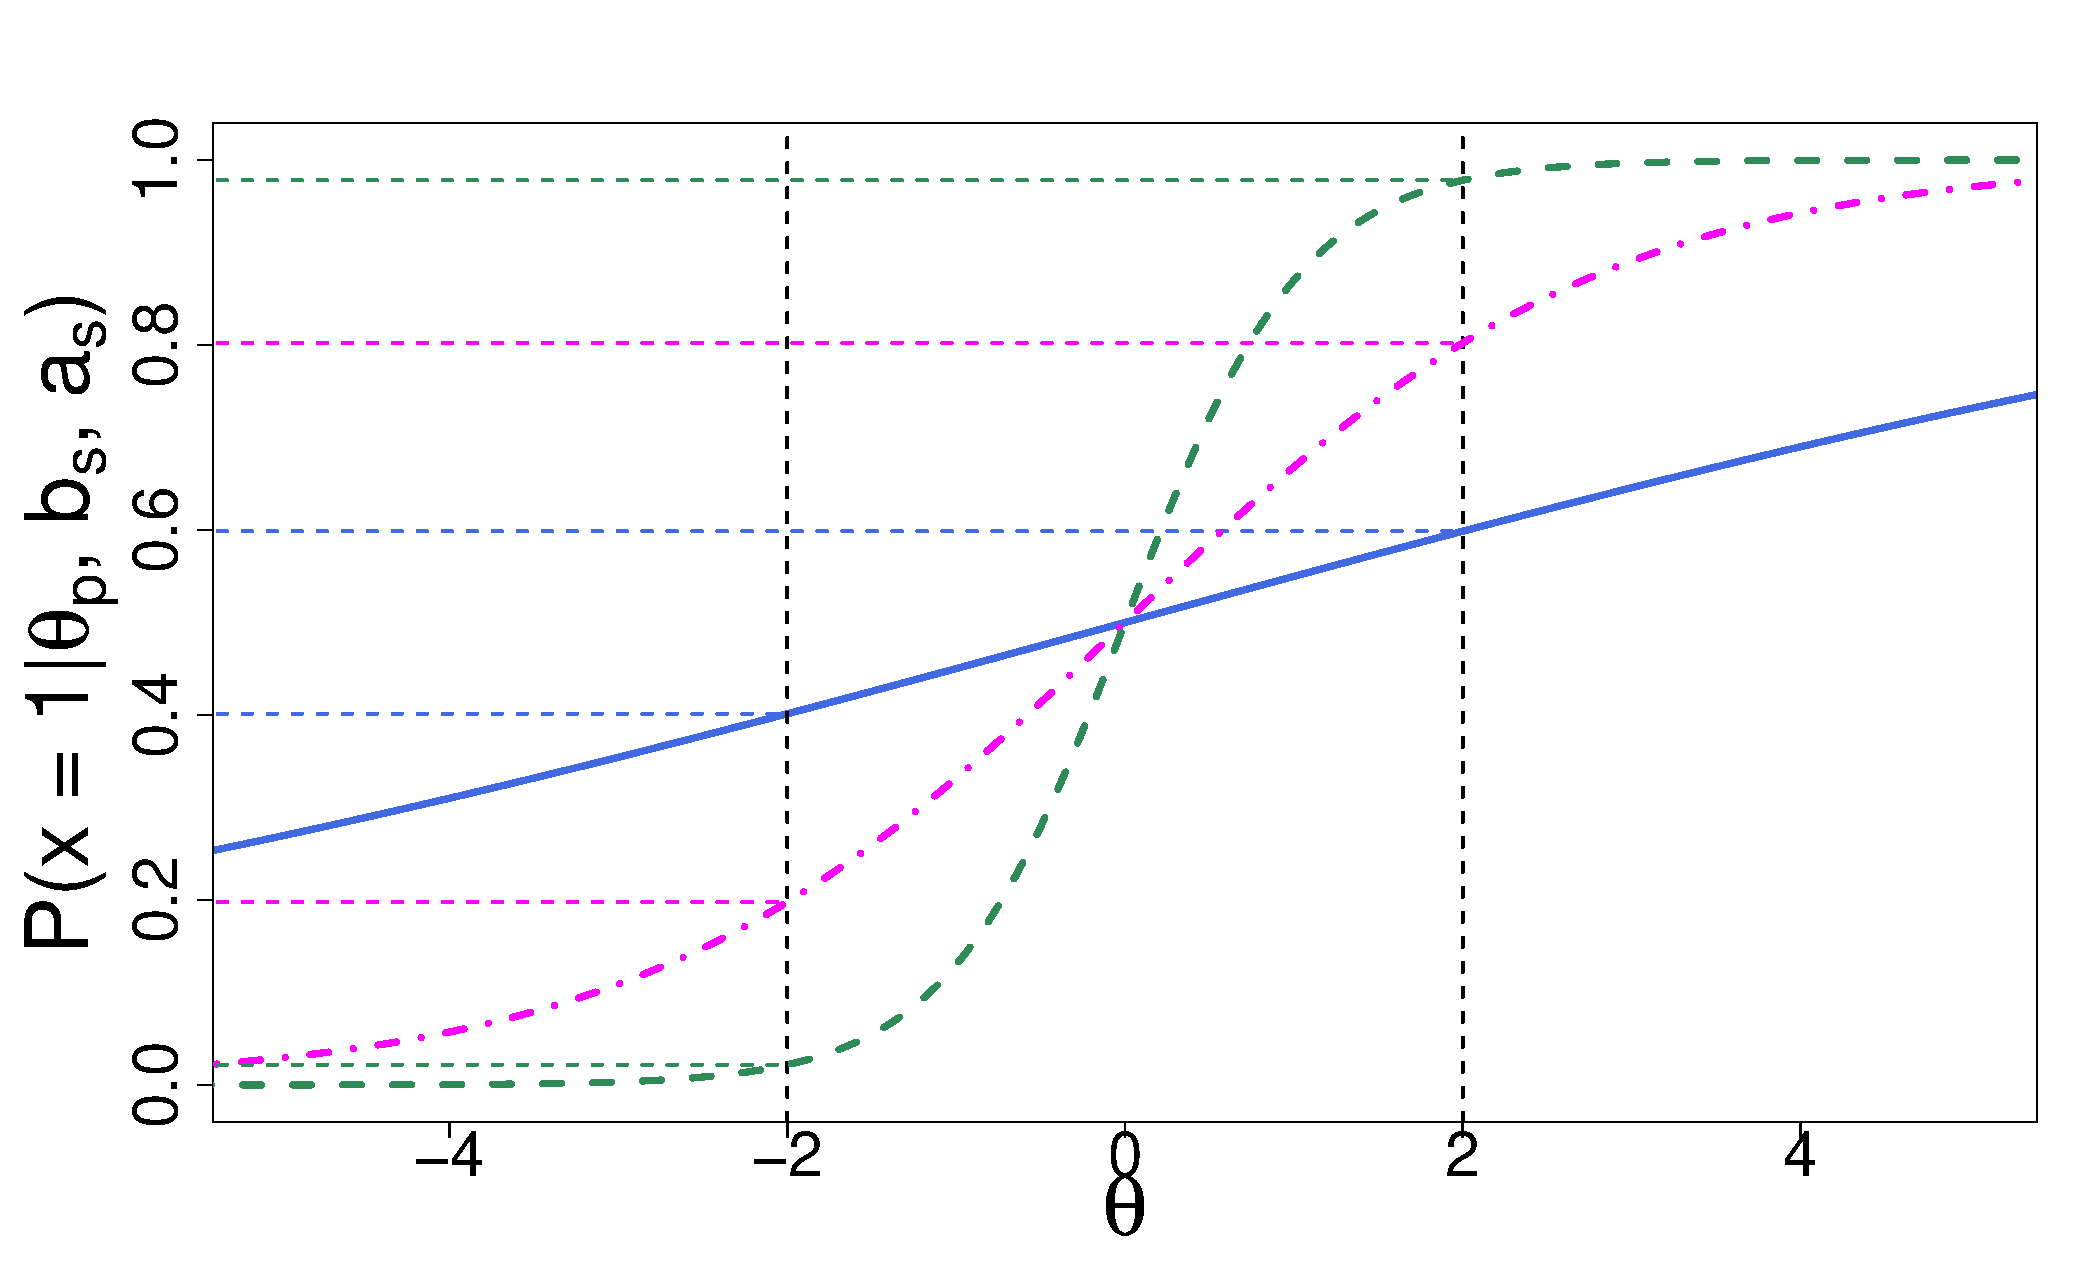
\includegraphics[width=\linewidth]{img/bs.pdf}
			\caption{Item Characteristics Curves (\emph{ICC}s) of items with $b=0$, and \textcolor{blue}{$a = 0.20$}, \textcolor{magenta}{$a = 0.70$}, 
				\textcolor{seagreen}{$a = 1.90$}}
			\label{sub:icc}
		\end{subfigure}
		\begin{subfigure}{.45\linewidth}
			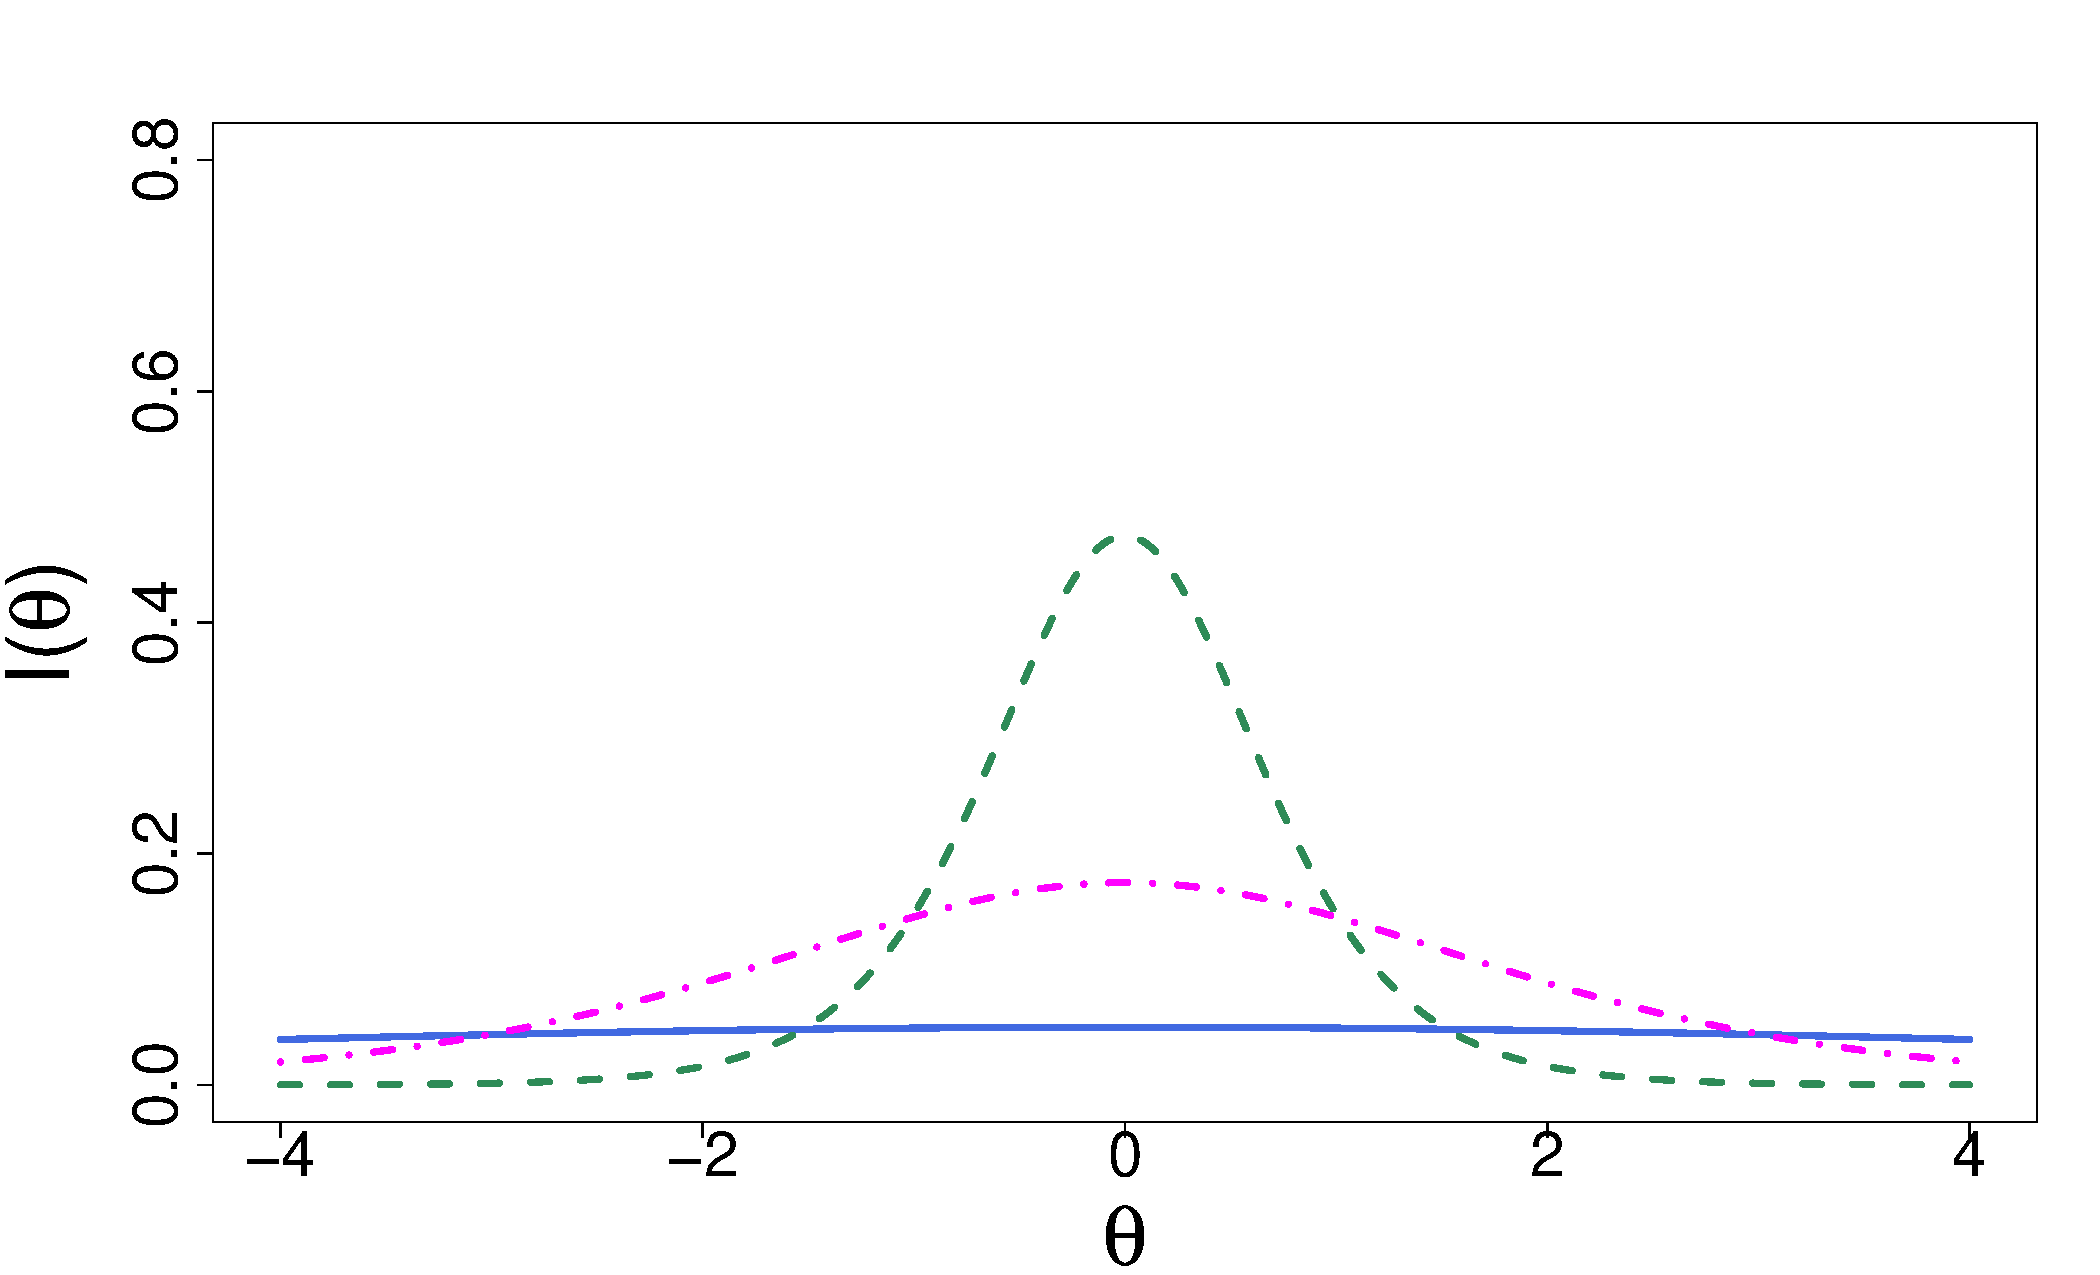
\includegraphics[width=\linewidth]{img/iifs.pdf}
			\caption{Item Information Functions (\emph{IIF}s) of items with $b=0$, and \textcolor{blue}{$a = 0.20$}, \textcolor{magenta}{$a = 0.70$}, 
				\textcolor{seagreen}{$a = 1.90$}}
			\label{sub:iif}
		\end{subfigure}
		
		\begin{subfigure}{.45\linewidth}
			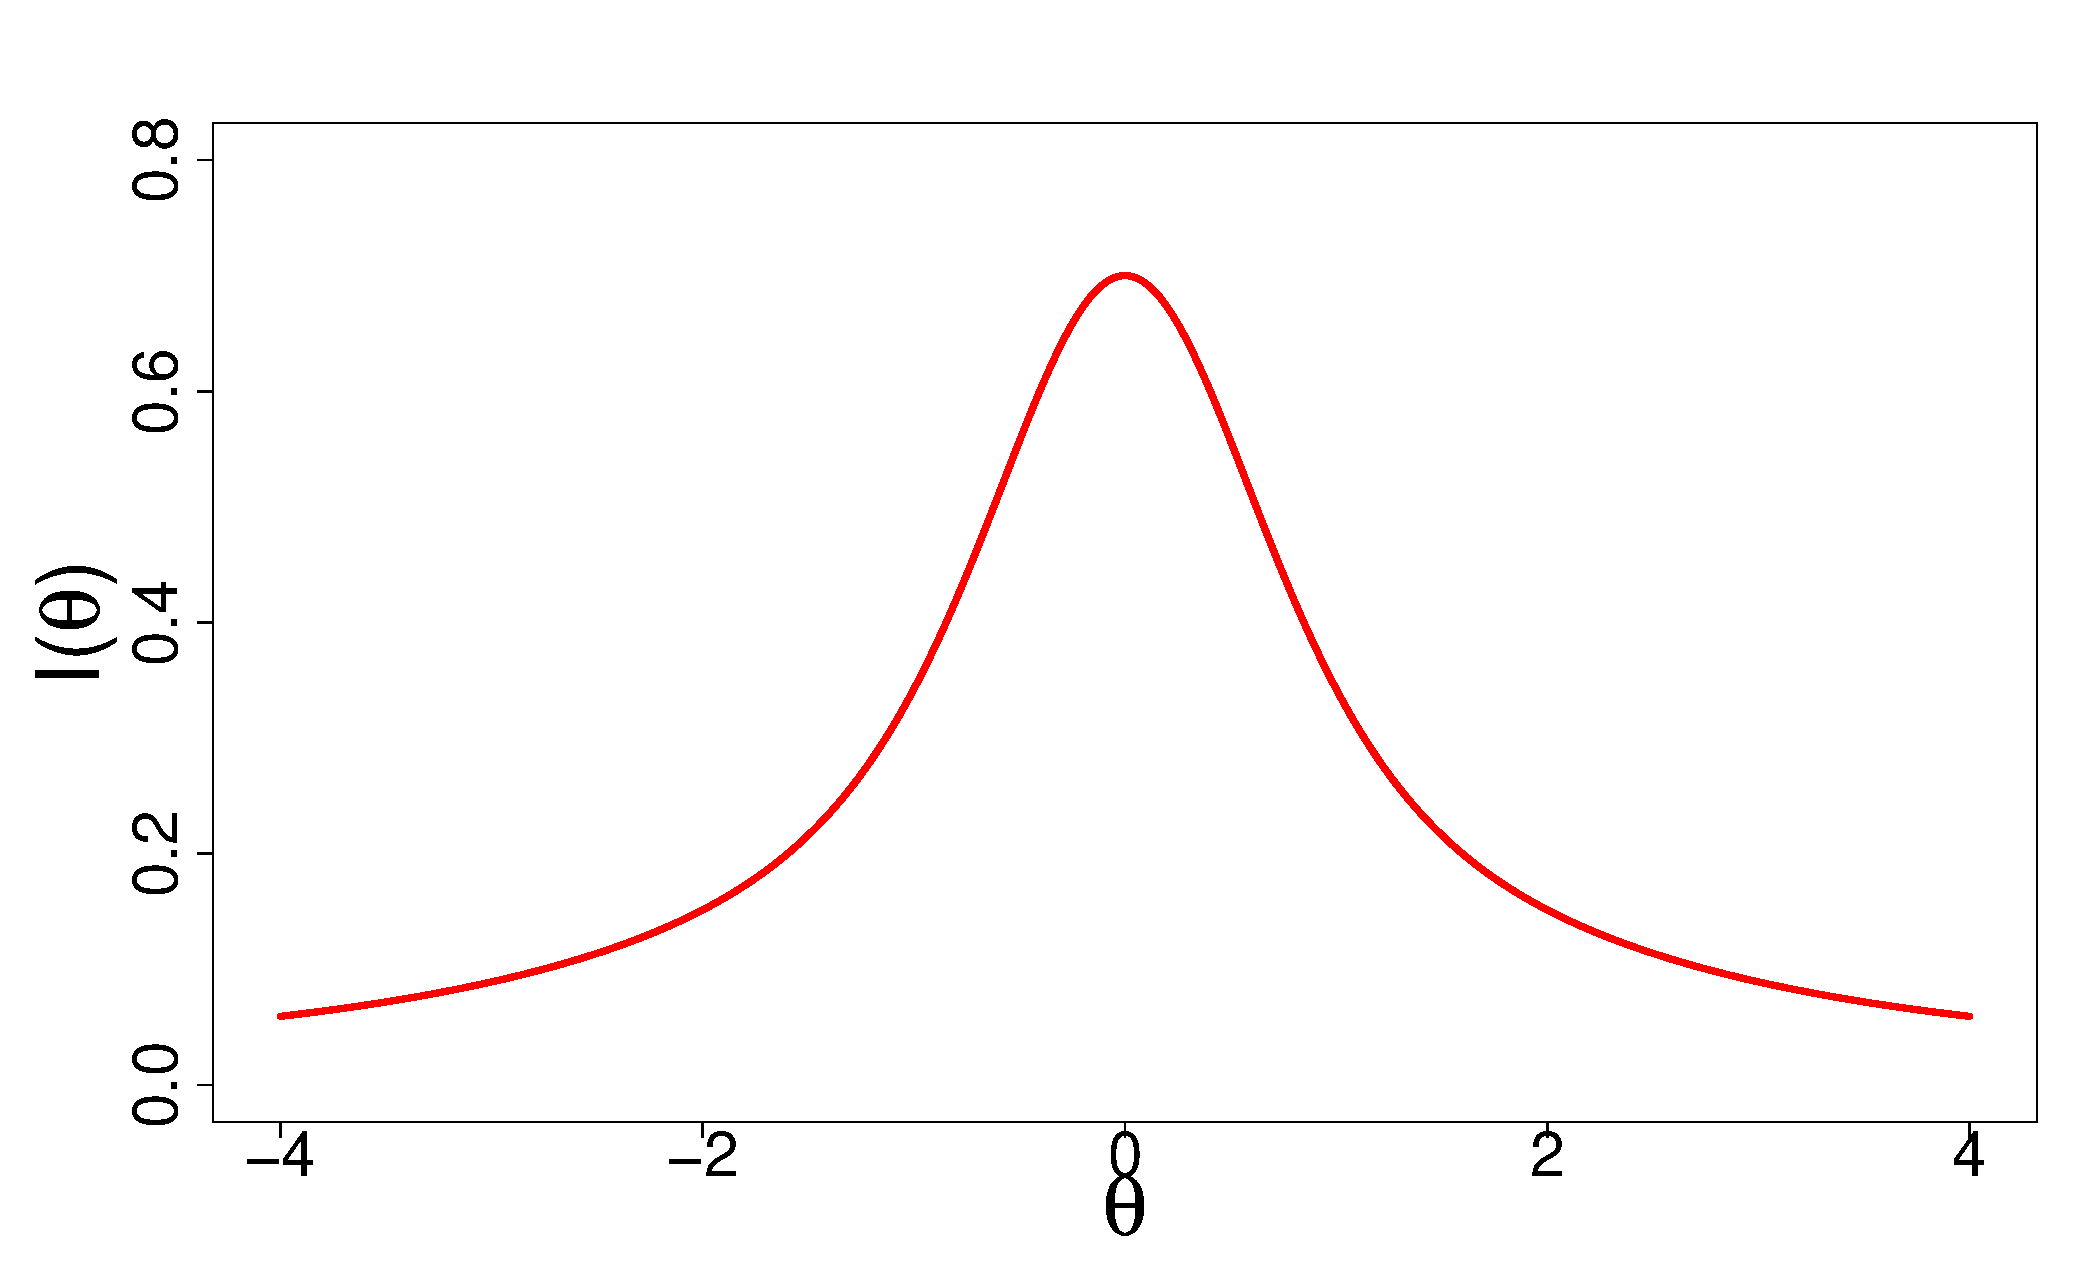
\includegraphics[width=\linewidth]{img/tif.pdf}
			\caption{Test Information Function (\emph{TIF}) of the test composed of the items in Fig. \ref{sub:icc} and Fig. \ref{sub:iif}.}
			\label{sub:tif}
		\end{subfigure}
		\caption{2-PL and information functions}
	\end{figure}
\end{block}
			
		
				

				
				\begin{block}{\centering Item Selection Procedures}
					 \begin{itemize}
					 	\item \textbf{Benchmark}: The $N$ items with the highest \emph{IIF}s are selected from the full-length test to be included in the static short form, where $N$ is the desired length of the short form (Benchmark Procedure, BP).
					 
					 	\item \textbf{Random}: Items are randomly selected from the full-length tests (RP).
					 	
					 	\item \textbf{Procedures based on $\theta'$}:
					 \end{itemize}
					 	\begin{quote}
					 		\begin{itemize}
					 			
					 			\item \textbf{Cluster}: The latent trait is clustered in $N$ clusters, where $n$ is the number of items to be included in the short form. The centroids of the clusters are the $\theta'$ (Unequal Intervals Procedure, UIP).
					 			
					 			\item \textbf{Intervals}: The latent trait is segmented into $N + 1$ intervals. Each interval is defined by $[\theta_{n-1}'; \, \theta_n']$. 
					 			The $\theta'$s are obtained by averaging between the lower and upper bound of each interval
					 			to avoid that the first and the last $\theta'$s correspond to the minimum and maximum $\theta$ values (Equal Intervals Procedure, EIP).
					 		\end{itemize}
					 	\end{quote}
		
					 
					Development of a 5-item short form from a 10-item full-length test: 
					\begin{columns}
						\begin{column}{.50\linewidth}
								\centering 
								Typical procedure
						\begin{table}[ht]
								\centering
								\begin{tabular}{rrrr}
									\hline
									item & $b$ & $a$ & \emph{IIF} \\ 
									\hline
							\rowcolor{template!20!}1	& $	-2.51	$ & $	1.68	$ & $	0.10	$ \\
							\rowcolor{template!20!}2	& $	-2.43	$ & $	0.25	$ & $	0.02	$ \\
							3	& $	-2.28	$ & $	1.62	$ & $	0.13	$ \\
							\rowcolor{template!20!}4	& $	-0.67	$ & $	0.71	$ & $	0.11	$ \\
							5	& $	-0.66	$ & $	0.44	$ & $	0.05	$ \\
							\rowcolor{template!20!}6	& $	0.50	$ & $	1.19	$ & $	0.27	$ \\
							7	& $	0.64	$ & $	0.50	$ & $	0.06	$ \\
						\rowcolor{template!20!}	8	& $	0.72	$ & $	0.33	$ & $	0.03	$ \\
							9	& $	1.72	$ & $	0.39	$ & $	0.03	$ \\
							10	& $	2.12	$ & $	1.98	$ & $	0.16	$ \\
							 
									\hline
								\end{tabular}
							\end{table}
						\end{column}
					
					\begin{column}{.50\linewidth}
						\centering $\theta'$-based procedures
						\begin{table}[ht]
							\centering
							\begin{tabular}{lrrrrr}
								\hline
								  & \textcolor{seagreen}{$\theta_1 $} & \textcolor{royalblue3}{$\theta_2 $} & \textcolor{template}{$\theta_3$} & \textcolor{typical}{$\theta_4$}& \textcolor{comp}{$\theta_5$ }\\ 
								 item			& \textcolor{seagreen}{$	-3.07	$} & \textcolor{seagreen}{$	-1.54	$ }& \textcolor{template}{$	-0.01	$} & \textcolor{typical}{$	1.53	$} & \textcolor{comp}{$	3.06	$} \\
								\hline
						1	& $	0.07	$ & $	0.12	$ & $	0.12	$ & $	0.07	$ & $	0.03	$ \\
				\textcolor{template}{2}	& $	0.02	$ & $	0.11	$ & \cellcolor{template!20!}$	0.32	$ & $	0.25	$ & $	0.06	$ \\
						3	& $	0.02	$ & $	0.02	$ & $	0.01	$ & $	0.01	$ & $	0.01	$ \\
						\textcolor{typical}{4}	& $	0.01	$ & $	0.01	$ & $	0.06	$ & 	\cellcolor{template!20!}$	0.71	$ & $	0.45	$ \\
						5	& $	0.02	$ & $	0.03	$ & $	0.03	$ & $	0.04	$ & $	0.03	$ \\
						\textcolor{royalblue3}{6}	& $	0.45	$ & \cellcolor{template!20!}$	0.46	$ & $	0.06	$ & $	0.01	$ & $	0.01	$ \\
						\textcolor{comp}{7}	& $	0.03	$ & $	0.05	$ & $	0.06	$ & $	0.06	$ & \cellcolor{template!20!}$	0.04	$ \\
						\textcolor{seagreen}{8}	& \cellcolor{template!20!}$0.57	$ & $	0.38	$ & $	0.04	$ & $	0.01	$ & $	0.01	$ \\
						9	& $	0.04	$ & $	0.05	$ & $	0.05	$ & $	0.04	$ & $	0.03	$ \\
						10	& $	0.02	$ & $	0.02	$ & $	0.03	$ & $	0.03	$ & $	0.02	$ \\
						\hline
			
						
							
							\end{tabular}
						\end{table}
					\end{column}
					\end{columns}
					
				
				\end{block}
				
			
			
				
			\end{column}
			
			%%%%%%%%%%%%%%%%%%%%%%%%%%%%%%%%%%%%%%%%%%%%%%%%%%%%%%%%%%%
			
			
			\begin{column}{.45\linewidth}
				
		\begin{block}{\centering Method}
			Comparison between the item selection procedures: 
			\begin{itemize}
				\item Benchmark procedure (BP)
				\item Unequal Intervals Procedure (UIP)
				\item Equal Interval Procedure (EIP)
				\item Random Procedure (RP)
			\end{itemize}
		in the development of 10, 30, 50, 70, 90 items test short forms from a  100-item full-length test \\
		(For each short test form, RP randomly selects the items 10 times).
			\begin{columns}
				\begin{column}{.50\linewidth}
					\begin{center}
						1000 respondents $p$
					\end{center}
					Three $\theta$ distributions: 
					\begin{enumerate}
						\item Normal distribution $p \sim \mathcal{N}(0,1)$
						\item Positive skewed distribution $p \sim Beta(1, 100)$ (linearly transformed to obtain negative values)
						\item Uniform distribution $p \sim \mathcal{U}(-3,3)$
					\end{enumerate}
					
				\end{column}
				
				\begin{column}{.50\linewidth}
					\begin{center}
						100 items $s$:
					\end{center}
					\begin{itemize}
						\item $b \sim \mathcal{U}(-3,3)$
						\item  $a \sim \mathcal{U}(0.40,2)$
					\end{itemize}
				\end{column}
			\end{columns}
	
	\end{block}
				
				\begin{block}{\centering Results}
					\begin{figure}
						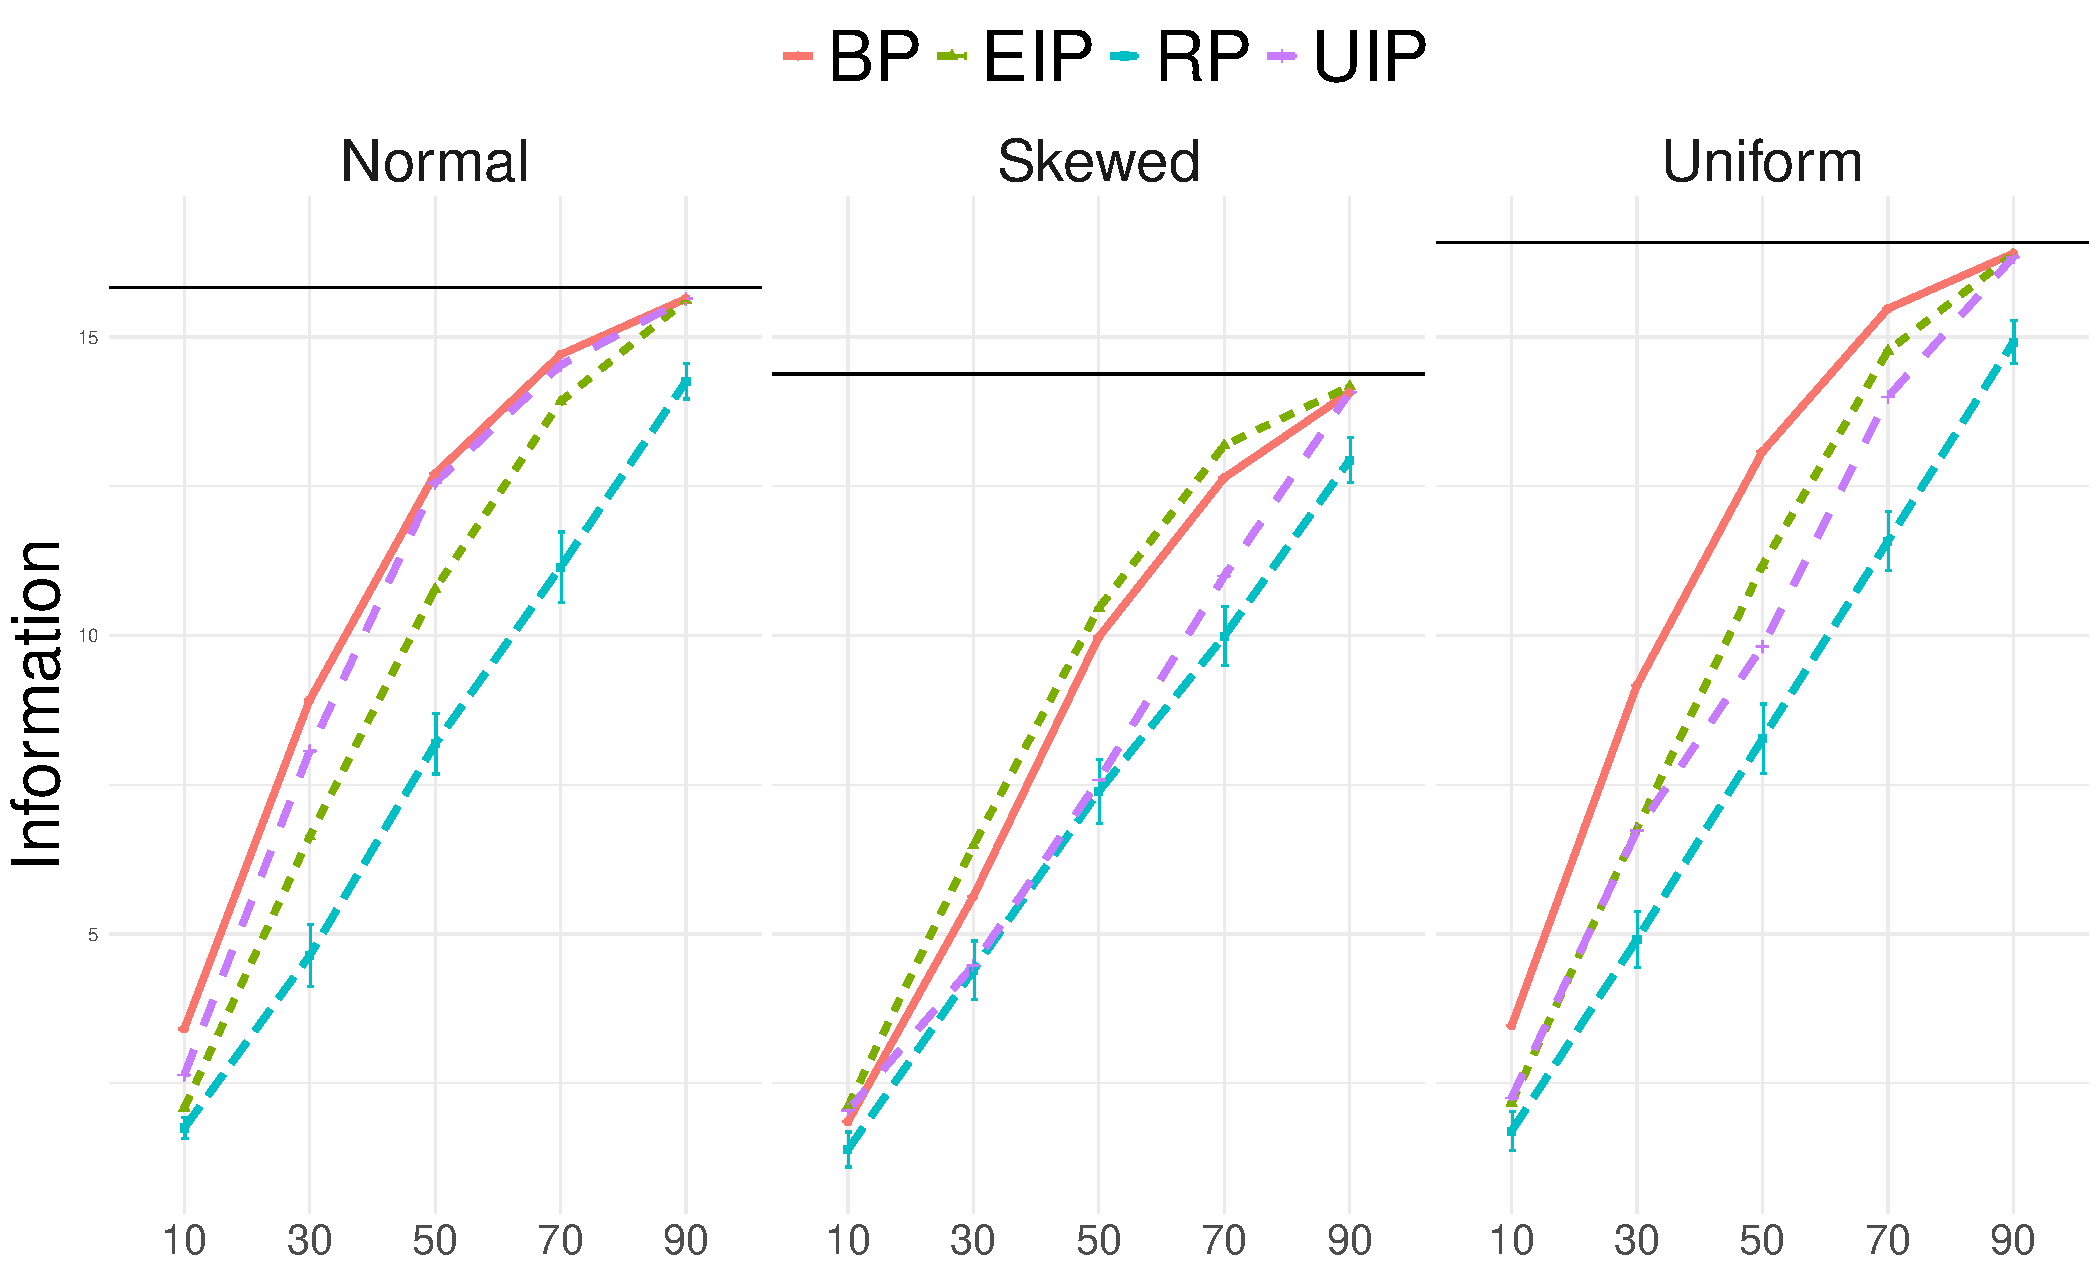
\includegraphics[width=\linewidth]{img/info.pdf}
						\caption{Overall information of the short test forms}
					\end{figure}
				
				\begin{figure}
					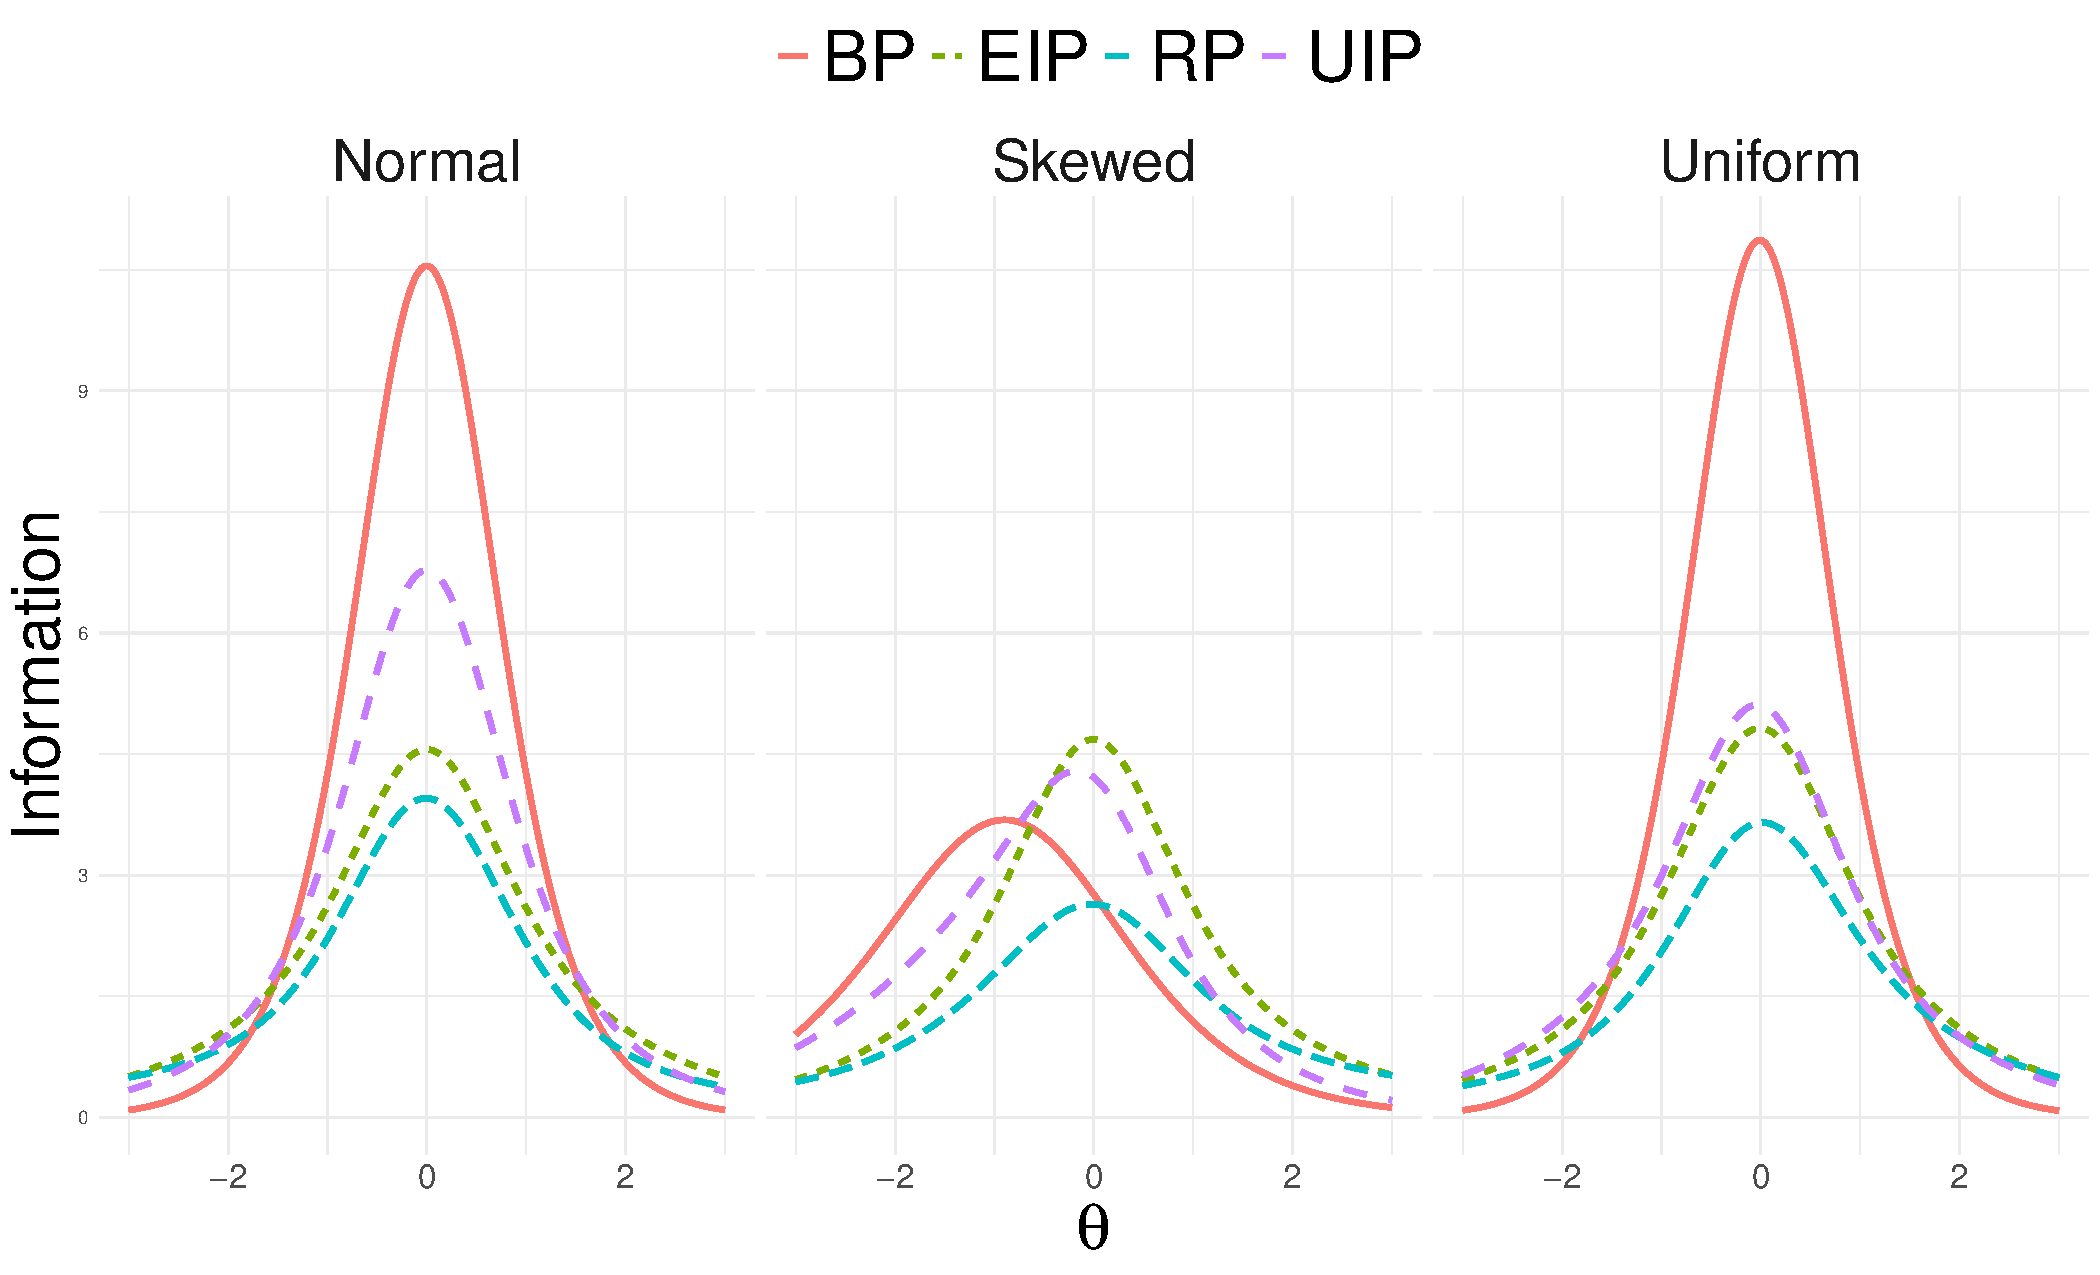
\includegraphics[width=\linewidth]{img/infoDetails.pdf}
					\caption{Detailed information of the short test forms}
				\end{figure}
			
				\begin{figure}
				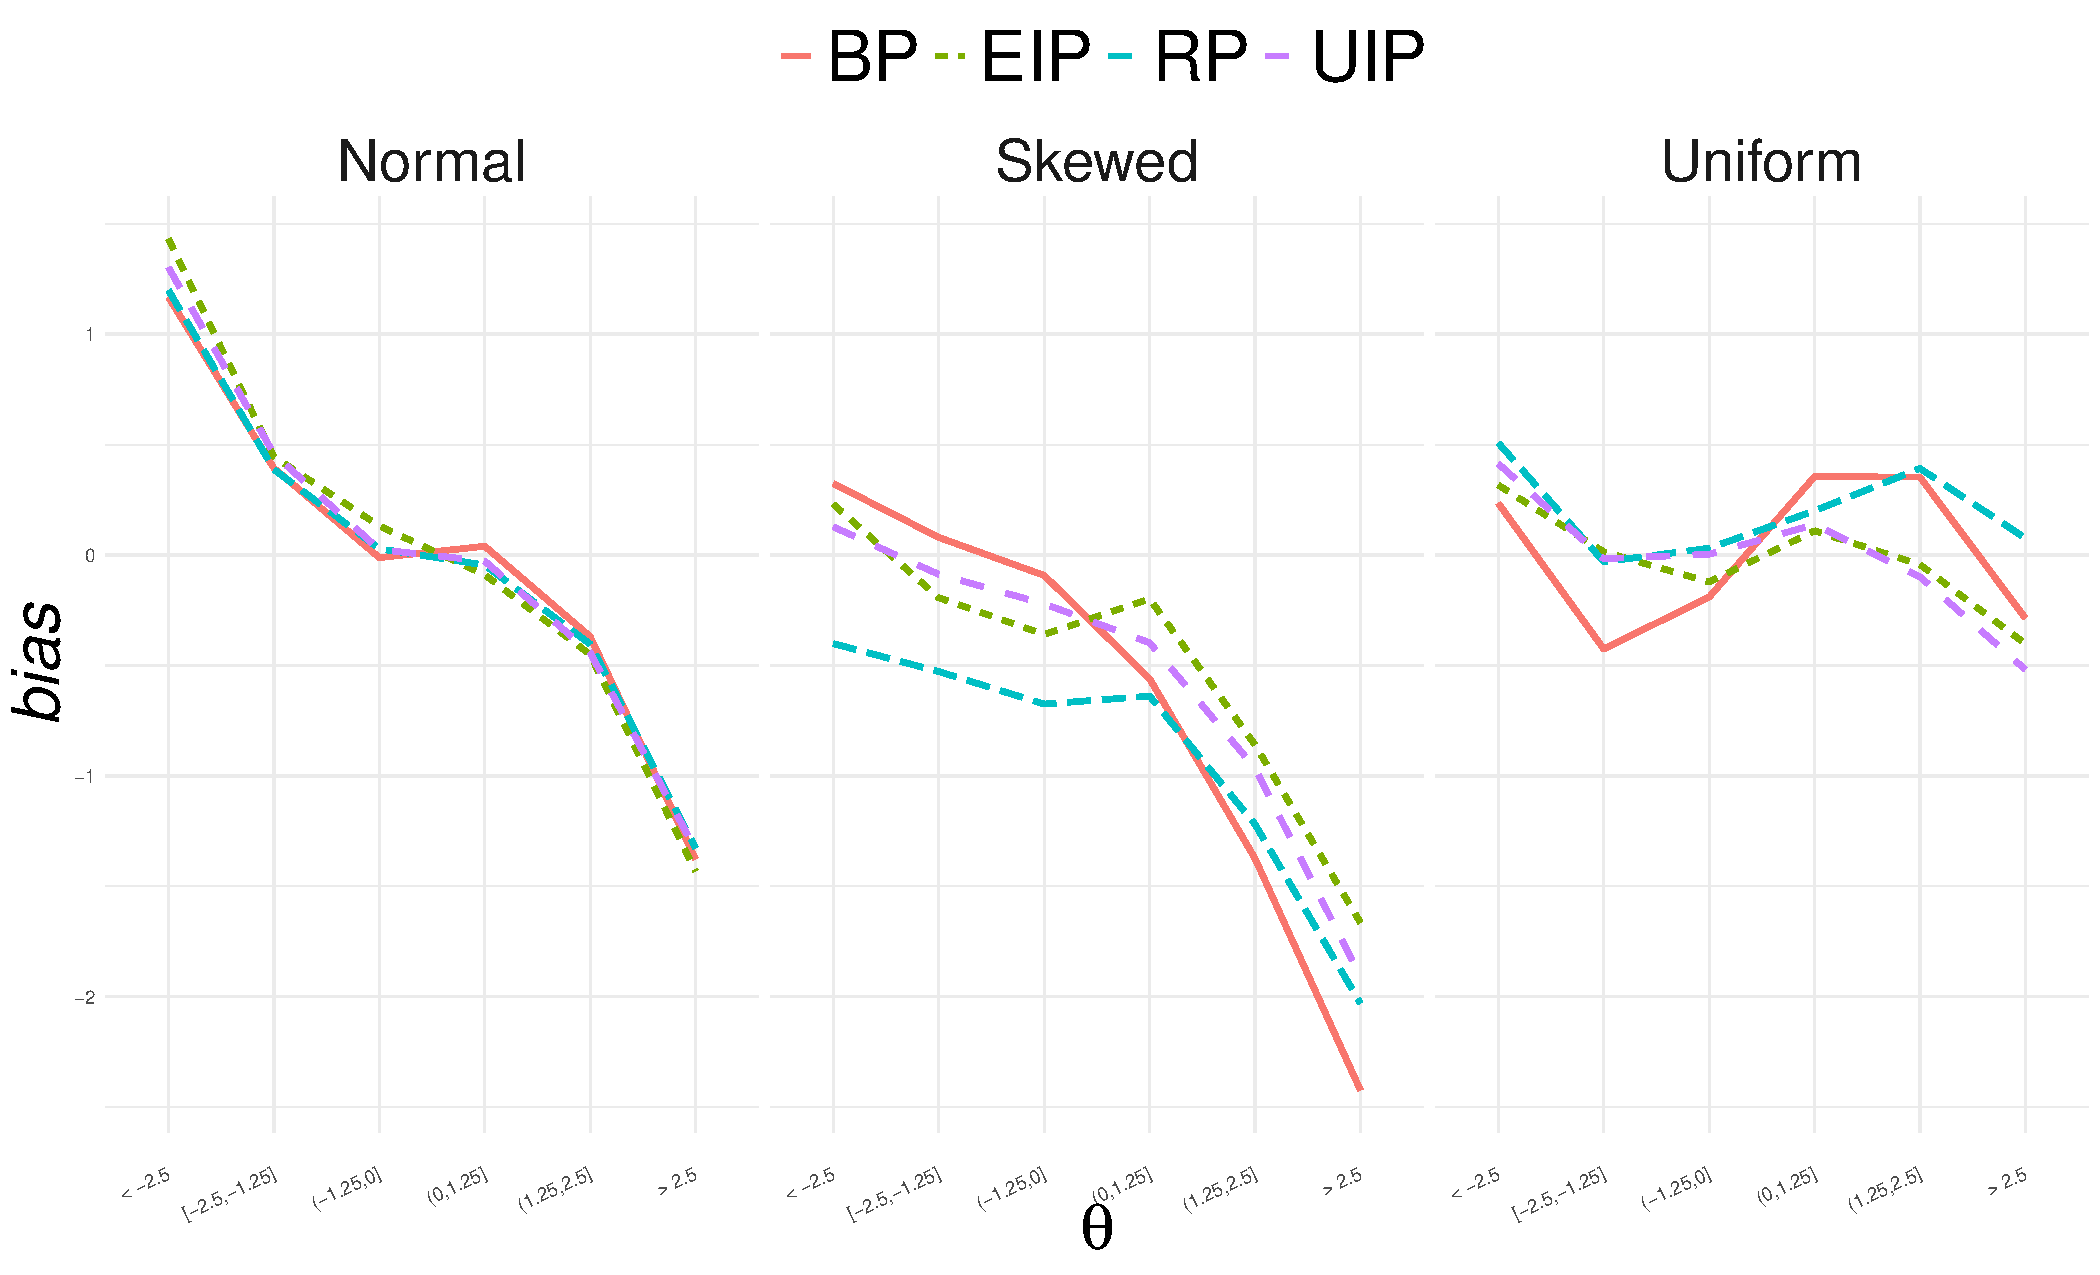
\includegraphics[width=\linewidth]{img/BIAS.pdf}
				\caption{Bias for different group of $\theta$}
			\end{figure}
				\end{block}
				
				\begin{block}{Discussion}
					\begin{itemize}
						\item Different methods for different $\theta$ distributions
						
						\item  Better performance of $\theta$-based procedures on the extreme ends of the distributions
						
						\item By considering the $\theta'$ in the item selection procedures $\rightarrow$ not the highest information but best coverage of the entire latent trait
					\end{itemize}

				\end{block}
			
	
				
			\end{column}
		\end{columns}
		
		
	\end{frame}
	
\end{document}
